\chapter{Collaboration Layer}
\label{chapter:collaborationlayer}

The collaboration layer is in between the two other layers: the network 
layer below and the application layer above. It is responsible for all the 
collaboration functionality. The code of the collaboration layer implementation
can be found in the package 
\texttt{ch.\-iserver.\-ace.\-collaboration.\-jupiter} and
its subpackages. The core responsibilities of this layer are:

\begin{itemize}
 \item host the concurrency control algorithm
 \item transform incoming as well as outgoing requests
 \item manage the set of participants in a given session
 \item access control
\end{itemize}

The concurrency control algorithm is based on the concept of operational 
transformation. It was developed and tested as part of the semester project.
In the diploma project, the main task in this layer was to integrate the
algorithm into the layer design documented in chapter 
\ref{chapter:archoverview}.

The collaboration layer can be split into different parts: a server part
and a client part. The client part differes significantly for a publisher
and a participant.



\section{CollaborationService}
The core entry point into the collaboration layer is an object implementing the
\texttt{Collaboration\-Service} interface. It is implemented by the
\texttt{Collaboration\-Service\-Impl} class, which also implements the
\texttt{Network\-Service\-Callback} interface. These interfaces and their
functionality have been thorougly explained elsewhere (see chapter 
\ref{chapter:archoverview}). 

The implementation of the collaboration service passes calls on 
the \texttt{Network\-Service\-Callback} methods to the corresponding
objects from the application
layer, namely the \texttt{User\-Listener}s, \texttt{Document\-Listener}s,
\texttt{Invitation\-Callback}, and \texttt{Service\-Failure\-Handler}.


\subsection{User and Document Management}
The collaboration service implementation delegates the management of the
set of currently discovered users and documents to objects implementing the
\texttt{User\-Registry} and \texttt{Document\-Registry} interface respectively.

The collaboration layer makes sure that for each unique user id there is
only one \texttt{Remote\-User}. Thus it is save to register a 
\texttt{Property\-Change\-Listener} on the 
\texttt{Remote\-User} to receive changes
to that user's name. It takes also care that there is only one 
\texttt{Remote\-Document} for a unique document id.

The \texttt{User\-Registry} manages the currently known set of users. The
objects registered in the registry are of type \texttt{Mutable\-Remote\-User},
an interface that adds a single method \texttt{set\-Name} to the 
\texttt{Remote\-User} interface. 
This method allows the collaboration layer to change the
name of a user, if such a change is reported from the network layer.
The \texttt{get\-User} method with an argument of type
\texttt{Remote\-User\-Proxy} creates a new \texttt{Mutable\-Remote\-User}, if 
a user with the same id does not already exist. Otherwise, the existing
user is returned. This makes sure that
there is only one \texttt{Remote\-User} object for a unique user. The
other \texttt{get\-User} method returns null if there is no user in the
registry with the given id.

\begin{figure}[H]
 \centering
 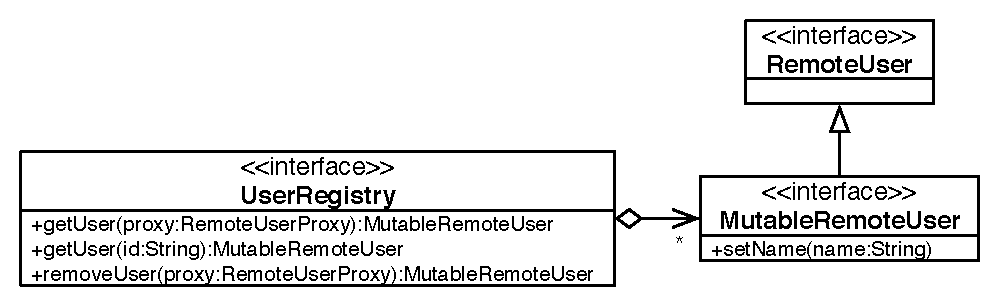
\includegraphics[width=15cm,height=4.23cm]{../images/finalreport/collaboration_userregistry_uml.eps}
 \caption{UserRegistry Interface}
 \label{fig:collaboration.userregistry}
\end{figure}

The \texttt{Document\-Registry} is the equivalent class for 
\texttt{Mutable\-Remote\-Document} objects. \texttt{Mutable\-Remote\-Document}
adds the \texttt{set\-Title} method to the \texttt{Remote\-Document}.

\begin{figure}[H]
 \centering
 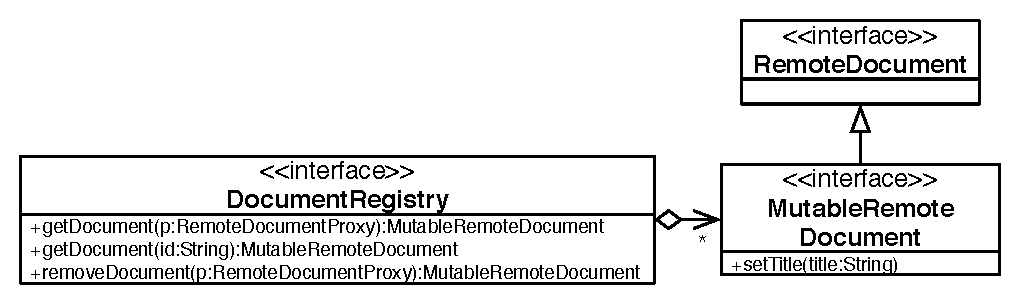
\includegraphics[width=15cm,height=4.12cm]{../images/finalreport/collaboration_documentregistry_uml.eps}
 \caption{DocumentRegistry Interface}
 \label{fig:collaboration.documentregistry}
\end{figure}

The mutable subinterfaces of \texttt{Remote\-User} 
and \texttt{Remote\-Document}
are never passed to the application layer, because the application layer
is never allowed to
change the name of other users or the title of documents published by other
users.



\section{Client Side}
The collaboration layer has to implement several interfaces defined in
the API to the adjacent layers.


\subsection{Receiving Invitations}
The collaboration layer has to implement the \texttt{Invitation} interface.
It is implemented by the \texttt{Invitation\-Impl} class. The implementation
is straightforward. The calls to \texttt{reject} and \texttt{accept} are
directly forwarded to the referenced \texttt{Invitation\-Proxy} from the
network layer. The only thing the collaboration layer does is wrap the
passed in \texttt{Join\-Callback} with an implementation of 
\texttt{Join\-Network\-Callback}.


\subsection{Join Callback}
To forward a join request to the network layer, the collaboration layer has
to implement the \texttt{Join\-Network\-Callback} interface. The
\texttt{accepted} method of the interface must create a \texttt{Session}
and pass that to the \texttt{Join\-Callback} of the application layer.
The callback returns a \texttt{Session\-Connection\-Callback} to the
network layer.


\subsection{Creating Sessions}
\texttt{Session} objects are created by a \texttt{Session\-Factory}. The
\texttt{Session\-Factory} creates \texttt{Configurable\-Session} objects, which
provide methods to set the \texttt{Session\-Connection} as well as the
\texttt{Participant\-Session\-Callback}.

\begin{figure}[H]
 \centering
 \includegraphics[width=8.89cm,height=4.73cm]{../images/finalreport/collaboration_uml.eps}
 \caption{Session factory and configurable session}
\end{figure}


\subsection{Participant Session}
The default implementation of the \texttt{Session} interface is the
\texttt{Session\-Impl} class. It implements the \texttt{Configurable\-Session}
interface, which also implements the \texttt{Session\-Connection\-Callback}
interface. So the implementation acts as both the \texttt{Session} to
the application layer as well as \texttt{Session\-Connection\-Callback} to the
network layer.

\subsubsection{Transformations}
The \texttt{Session\-Impl} class hosts the client-side transformation algorithm.
Every received request is transformed with that algorithm. Before a
received request can be transformed, the session has to be locked (locking
the lock passed from the application layer by the \texttt{get\-Lock} method
of the \texttt{Session\-Callback}). When sending operations, the algorithm
is used to create a request that can be sent to the 
\texttt{Session\-Connection}.

\subsubsection{Session Connection Handling}
The \texttt{Configurable\-Session} has a method called \texttt{set\-Connection},
which passes the \texttt{Session\-Connection} to the \texttt{Session}. The
\texttt{Session\-Impl} makes use of a \texttt{Thread\-Domain} (see
appendix \ref{chapter:threaddomains}) to execute calls on that 
\texttt{Session\-Connection} asynchronously. The main reason for doing this
is that the caller thread (most likely the AWT event dispatch thread)
is not slowed down by a potentially slow network connection. The caller thread 
can go on and execute other tasks.

However, using asynchronous calls has one significant
disadvantage. Exceptions thrown by the method invocation cannot be
thrown back at the caller (i.e. the application layer). That is where
the \texttt{Session\-Connection\-Wrapper} helps out. It is an implementation
of the \texttt{Session\-Connection} interface that catches all exceptions
thrown by the target \texttt{Session\-Connection} and passes them to an
object implementing the \texttt{Session\-Connection.Failure\-Handler}
interface. The figure \ref{fig:collaboration.sessionconnectionwrapper}
shows exactly the described setup.

\begin{figure}[H]
 \centering
 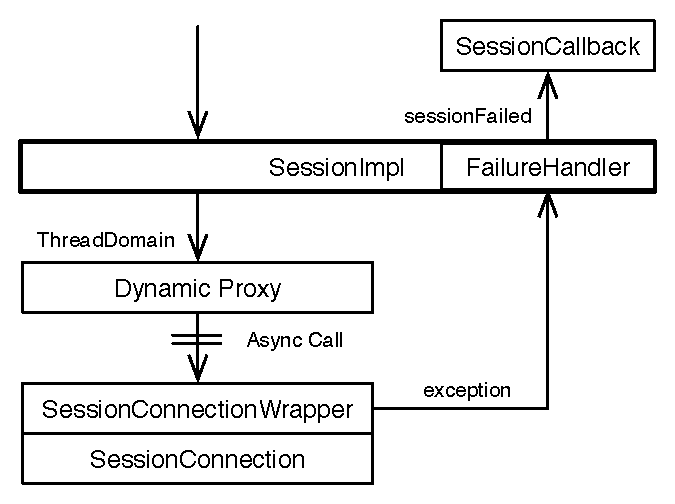
\includegraphics[width=9.77cm,height=7.58cm]{../images/finalreport/collaboration_sessionconnectionwrapper.eps}
 \caption{Wrapped session connection with ThreadDomains}
 \label{fig:collaboration.sessionconnectionwrapper}
\end{figure}

The call from the dynamic proxy to the \texttt{Session\-Connection\-Wrapper}
is asynchronous. The methods of the \texttt{Session\-Connection\-Wrapper}
are executed by a designated worker thread (see the little circle in the
figure \ref{fig:collaboration.sessionconnectionwrapper}). If the target 
\texttt{Session\-Connection} throws an exception, the wrapper catches
it and invokes the method 
\texttt{handle\-Failure} on the \texttt{Failure\-Handler}. The
\texttt{Session\-Impl} implements the \texttt{Failure\-Handler} interface and
passes the failure to the \texttt{Session\-Callback}. A session that failed
once cannot be used any longer. 

\subsubsection{Acknowledge Messages}
The \texttt{Session\-Impl} uses a \texttt{Acknowledge\-Strategy} to determine
when to send acknowledge messages. For details about acknowledge strategies
see the section \ref{sect:archoverview.acknowledgestrategies}.

\small{\begin{verbatim}
  Timestamp timestamp = getAlgorithm().getTimestamp();
  int siteId = getAlgorithm().getSiteId();
  getConnection().sendAcknowledge(siteId, timestamp);
\end{verbatim}}

The preceding code snippet shows the implementation of the 
\texttt{Acknowledge\-Action}. The code is rather straightforward. It just
invokes the \texttt{send\-Acknowledge} method on the 
\texttt{Session\-Connection}.


\subsection{Published Session}
The publisher of a document gets a \texttt{Published\-Session} object from
the \texttt{publish} method of the \texttt{Collaboration\-Service}. The
implementation of this interface is the \texttt{Published\-Session\-Impl}
class, which, as we have seen, implements the \texttt{Publisher\-Connection}
interface too.

The published session hosts the client-side algorithm of the publisher.
It also has a reference to a \texttt{Acknowledge\-Strategy}, which is
used to send acknowledge strategies (see section 
\ref{sect:archoverview.acknowledgestrategies}).

\begin{figure}[H]
 \centering
 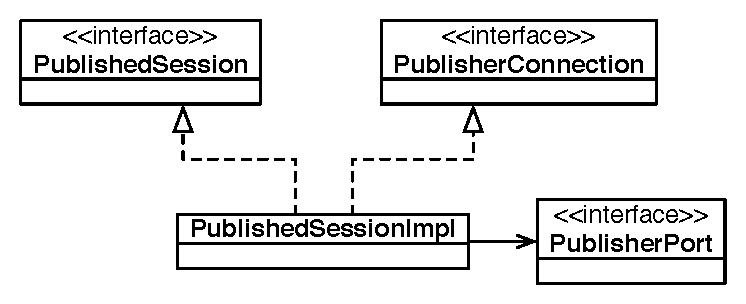
\includegraphics[width=12.67cm,height=4.59cm]{../images/finalreport/collaboration_publishedsession_uml.eps}
 \caption{PublishedSession implementation}
 \label{fig:collaboration.publishedsession}
\end{figure}

The implementation of the \texttt{Published\-Session} uses a
\texttt{Participant\-Port} to send events to the server-side of the session.



\section{Session Server} 
First of all, to avoid any confusion. The server part in the collaboration
layer has nothing to do with a network layer server, for instance a Java
application listening on a \texttt{Server\-Socket}. The collaboration layer
server is a purely logical construct. In this chapter we refer to
this collaboration layer server simply as server.

For each session, there must be one (logical) session server. It
hosts the server part of the concurrency control algorithm
(see chapter \ref{chapter:algorithm}). Further
it controls who joins the session and ensures that the session's list of
participants is kept up-to-date. The server itself does not have a graphical
user interface. At the moment, the session server runs inside the same JVM
as the publisher's application layer.


\subsection{Overview}
For each published document there is an object implementing the
\texttt{Server\-Logic}�interface. This interface extends the
\texttt{Document\-Server\-Logic} interface with methods only visible to the
collaboration layer itself. The only implementation of it is
\texttt{Server\-Logic\-Impl}.

Incoming communication from a particular participant is coming through an
implementation of the \texttt{Participant\-Port} interface. The 
\texttt{Participant\-Port} represents the entry point for messages from
one particular participant into the server. Outgoing communication happens 
through an implementation of \texttt{Participant\-Connection}, which is provided 
by the network layer. This interface is used by the collaboration
layer to send messages to one particular participant. For every participant, 
there is such a pair of objects. 

\begin{figure}[H]
 \centering
 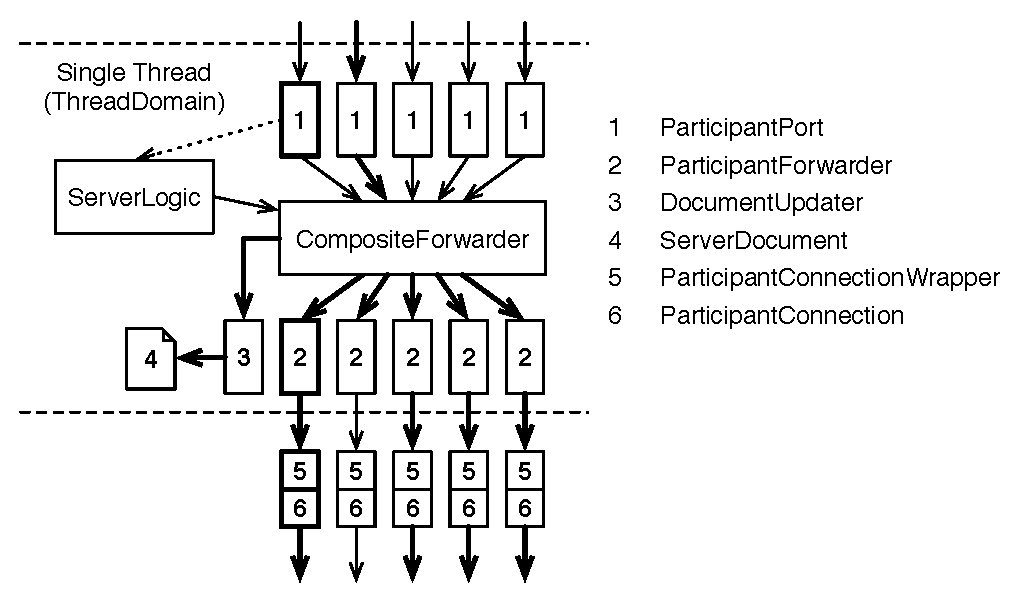
\includegraphics[width=15.56cm,height=7.9cm]{../images/finalreport/collaboration_serverflow.eps}
 \caption{Collaboration Layer Server}
 \label{fig:collaboration.serverflow}
\end{figure}

The server acts as a delivery station for messages from participants. 
Incoming requests are transformed by the corresponding 
\texttt{Participant\-Port} (1).
The resulting operation is passed to the \texttt{Composite\-Forwarder}, which in 
turn gives the request to all its child \texttt{Forwarders} (2 and 3). One child
forwarder is responsible to keep an up-to-date version of the document, whose
name is \texttt{Document\-Updater} (3). The \texttt{Document\-Updater} updates
a \texttt{Server\-Document} (4).

The other forwarders are \texttt{Participant\-Forwarder}s (2). They generate
requests, by using the server-side \texttt{Algorithm} for the corresponding
participant. The generated request is passed to a 
\texttt{Participant\-Connection}.

Objects assigned to the same participant are aligned vertically. So the
objects 1, 2, and 5 that are aligned vertically belong all to the
same participant. One participant is the publisher of the document. 
\texttt{Participant\-Port} and \texttt{Participant\-Forwarder} for a
particular participant have a reference to the server-side algorithm for
that participant.

The processing in the server from the point where a request crosses the
dashed line at the top to the point where all resulting requests have passed
the dashed line at the bottom must be sequential. This goal is achieved by
use of a \texttt{Single\-Thread\-Domain} (see section 
\ref{sect:collaboration.threaddomains}).

\subsubsection{Example}
The bold arrows represent a request as it passes through the server. First,
it is received by the second \texttt{Participant\-Port} from the left. Then it 
is passed
to the \texttt{Composite\-Forwarder}, which forwards the request to all
its children. The \texttt{Participant\-Forwarder} (2) for the same 
participant filters the message (the sender does not want
to receive his own messages).
All the other \texttt{Forwarder}s pass the
message on to the \texttt{Participant\-Connection} (5) (or to the
\texttt{Server\-Document} (4) in case of the \texttt{Document\-Updater} (3)).


\subsection{Server Logic}
The \texttt{Server\-Logic} provides methods that allows users to join,
participants to leave, setting the document details, inviting users as well
as shutting down the server logic. The interface is depicted in figure 
\ref{fig:collaboration.serverlogic}. 

\begin{figure}[H]
 \centering
 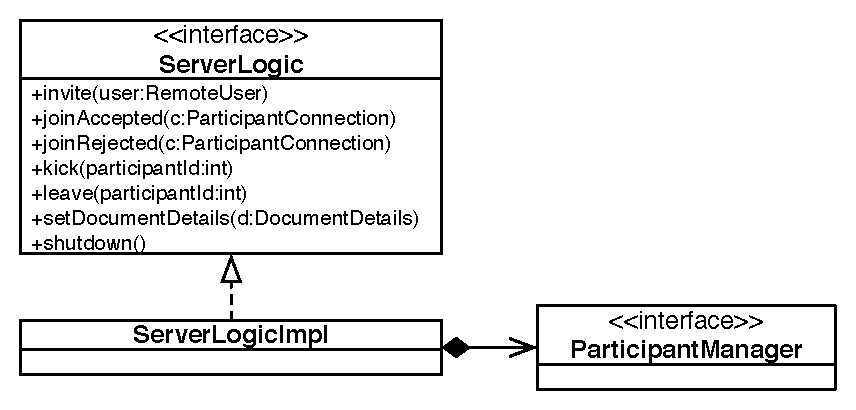
\includegraphics[width=13.93cm,height=6.39cm]{../images/finalreport/collaboration_serverlogic_uml.eps}
 \caption{ServerLogic Interface}
 \label{fig:collaboration.serverlogic}
\end{figure}

The \texttt{invite} method allows to invite a \texttt{Remote\-User} to
the session. The inherited \texttt{join} method from the
\texttt{Document\-Server\-Logic} interface allows the network layer to send
join requests. The \texttt{join\-Accepted} and \texttt{join\-Rejected} methods
notify the logic that a join request was accepted or rejected. 

The \texttt{kick} method allows to kick the participant with the given
id from the session. A kicked user is blacklisted, he
can no longer join the session. 

The \texttt{leave} method notifies the
server logic that the participant identified by the given id left the
session. 

The \texttt{set\-Document\-Details} method provides a way to change the
title of the document. This is used when the publisher saves the document
with a different name.

Finally, the \texttt{shutdown} method must be called when the session is
concealed by the publisher. It causes the server to properly dispose
all resources used by it.

\subsubsection{Participant Management}
The server logic implementation delegates the management of participants
to a class implementing the \texttt{Participant\-Manager} interface. This
class is consulted to determine which users are currently in the
session (\texttt{is\-Participant}), whether a user is blacklisted 
(\texttt{is\-Blacklisted}), whether the user has already sent a join
request which was not answered yet (\texttt{is\-Joining}), and whether a
user has been invited (\texttt{is\-Invited}).

Blacklisted users are no longer allowed to join the session unless they
are invited by the publisher. A join request from a user that 
issued already an unanswered join request is rejected too. This is needed
to prevent the same user joining the session twice.

\begin{figure}[H]
 \centering
 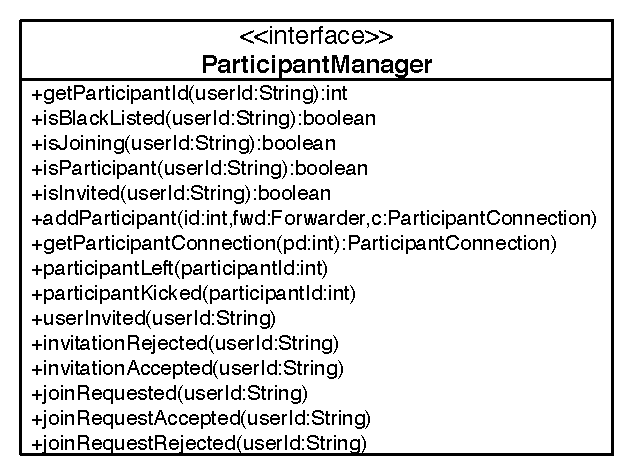
\includegraphics[width=10.16cm,height=7.48cm]{../images/finalreport/collaboration_participantmanager_uml.eps}
 \caption{ParticipantManager Interface}
 \label{fig:collaboration.participantmanager}
\end{figure}

The method \texttt{get\-Participant\-Id} is used to assign a user a participant
id. An implementation can assign a user that joins, leaves, and
rejoins the same session to assign the same participant id. The
\texttt{add\-Participant} method is used to add a participant to the
session. The \texttt{get\-Participant\-Connection} allows to get the 
\texttt{Participant\-Connection} for a participant.

The other methods exist to notify the \texttt{Participant\-Manager} about
participant related events. An implementation of this interface can use
these methods to keep the internal data structures up-to-date. The
default implementation is \texttt{Participant\-Manager\-Impl}.

\subsubsection{Join Requests}
When a user tries to join, the request is encapsulated in an object
implementing the \texttt{Join\-Request} interface. The \texttt{Join\-Request}
is then passed to the publisher through the \texttt{Publisher\-Connection}
(see section \ref{sect:archoverview.publisherconnection}).

The \texttt{Join\-Request} interface is
implemented by the \texttt{Join\-Request\-Impl} class. The implementation
is rather straightforward. The \texttt{accept}�method is passed to
the \texttt{join\-Accepted} method of the \texttt{Server\-Logic} interface.
The \texttt{reject} method is passed to the \texttt{join\-Rejected}
method of the \texttt{Server\-Logic} interface.

\subsubsection{Failure Handling}
\label{sect:collaboration.failurehandling}
The \texttt{Server\-Logic} needs a solid failure handling, otherwise it can
easily happen that the replicas start to diverge. The interface
\texttt{Failure\-Handler} is used to handle failures in the server logic. 

\begin{figure}[H]
 \centering
 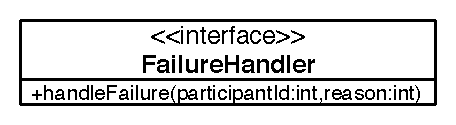
\includegraphics[width=7.16cm,height=1.55cm]{../images/finalreport/collaboration_failurehandler_uml.eps}
 \caption{FailureHandler Interface}
 \label{fig:collaboration.failurehandler}
\end{figure}

It is passed to all objects where errors can potentially occur. The failure
handler is passed to the following places.

\begin{itemize}
 \item participant ports
 \item \texttt{ParticipantConnectionWrapper}
 \item \texttt{CompositeForwarderImpl}
\end{itemize}

The \texttt{Server\-Logic\-Impl} implements that interface. The 
\texttt{handle\-Failure} method has a participant id parameter. That parameter
is used to determine to which participant the failure is related. If
it is a normal participant, that participant is removed from the session
and all other participants are notified about the participant that left.

However, if the failing participant is the publisher, the session is
terminated. In the current implementation of ACE, the publisher is always
in the same Java Virtual Machine as the server logic. Thus, there should
never really be a failure. If there is, it is most likely a bug in the
implementation, from which we cannot recover.



\subsection{Participant Port}
Objects implementing the \texttt{Participant\-Port} interface are used 
by the network layer to pass messages from one participant to the
server logic (see figure \ref{fig:archoverview.participantport}). 
The implementation of that interface is 
\texttt{Participant\-Port\-Impl}. The participant port has a reference to
the server-side algorithm for the participant. Received requests are
transformed by use of the server-side algorithm and the resulting
operation is forwarded to a \texttt{Forwarder}.

The \texttt{leave} method of the \texttt{Participant\-Port} interface is
forwarded to the \texttt{leave} method on the \texttt{Server\-Logic}. 


\subsubsection{Publisher Port}
\label{sect:archoverview.publisherport}
The interface \texttt{Publisher\-Port} extends the \texttt{Participant\-Port}
with methods only available to the publisher of the document. 

\begin{figure}[H]
 \centering
 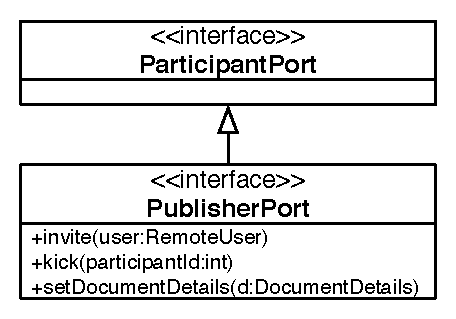
\includegraphics[width=7.16cm,height=4.83cm]{../images/finalreport/collaboration_publisherport_uml.eps}
 \caption{PublisherPort Interface}
 \label{fig:collaboration.publisherport}
\end{figure}

The \texttt{kick} method provides the publisher of the session a way to kick
one particular participant from the session. A kicked user is blacklisted
and no longer allowed to join the session (unless the publisher invites
him again).

The \texttt{invite} method is used to invite a user to the session and finally,
the \texttt{set\-Document\-Details} method makes it possible to change the 
document title (for instance if the document is renamed).

The default implementation of the \texttt{Publisher\-Port} interface is
the \texttt{Publisher\-Port\-Impl} class. The implementation has a direct
reference to the \texttt{Server\-Logic} as well as to the \texttt{Forwarder}
of the session.

\subsubsection{Failure Handling}
The participant ports transform incoming requests. If a request cannot
be transformed because it is invalid, the algorithm throws an exception.
This exception is caught by the participant ports and the participant
is expelled from the session. First, a participant that sends invalid requests
is not an acceptable participant, and second that particular participant
has an invalid document state. The operation has been applied locally but
the server rejected the corresponding request. Thus, the document state of
that particular participant starts to diverge from the correct document
content and so can no longer be part of the session.


\subsection{Forwarders}
We have already heard of the \texttt{Composite\-Forwarder} interface, which
represents a specialized version of the more general \texttt{Forwarder}
interface.

\begin{figure}[H]
 \centering
 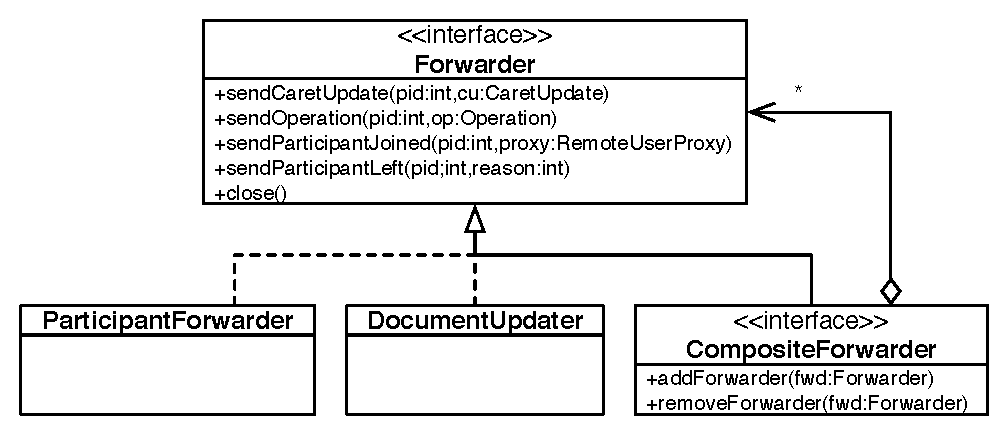
\includegraphics[width=16.51cm,height=6.81cm]{../images/finalreport/collaboration_forwarder_uml.eps}
 \caption{Forwarder inheritance hierarchy}
 \label{fig:collaboration.forwarder}
\end{figure}

A \texttt{Forwarder} receives messages processed by a 
\texttt{Participant\-Port}. For
instance if a request from a participant is received, the transformed
operation is passed to the \texttt{send\-Operation} method. Similar, there
is a \texttt{send\-Caret\-Update} method for \texttt{Caret\-Update}s. 
Additionally
there are two methods that notify the \texttt{Forwarder} about participation
events. The \texttt{close} method is called when the \texttt{Forwarder}
is no longer needed.

\subsubsection{CompositeForwarder}
\label{sect:collaboration.compositeforwarder}
The \texttt{Composite\-Forwarder} is used by the implementation of the
server logic to send the events described above to a collection of
\texttt{Forwarder} objects. This interface adds methods to add and
remove \texttt{Forwarder} objects from the list of forwarders of the
\texttt{Composite\-Forwarder}. The only implementation of that
interface is \texttt{Composite\-Forwarder\-Impl}.

The \texttt{Composite\-Forwarder\-Impl} knows the concept of a default
forwarder. The default forwarder is a \texttt{Forwarder} that receives
all events as first forwarder. If the default forwarder throws an
exception, the event is not forwarded to the other forwarders. Instead
a \texttt{Failure\-Handler} is notified, which determines what to do
with that failure. The default forwarder used is described in 
section \ref{sect:archoverview.documentupdater}.

\subsubsection{ParticipantForwarder}
The \texttt{Participant\-Forwarder} has a reference to the server-side algorithm
for one participant. There is a \texttt{Participant\-Forwarder} for each
participant in the session. This type of forwarder generates requests for
the operations obtained through the \texttt{send\-Operation} method and 
forwards them to the \texttt{Participant\-Connection} of that particular
participant. Similarly it generates a \texttt{Caret\-Update\-Message} for
a \texttt{Caret\-Update}.

\begin{figure}[H]
 \centering
 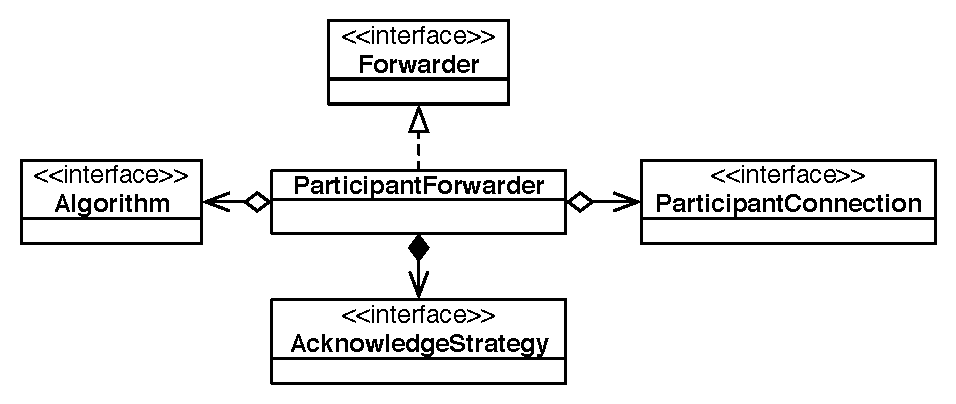
\includegraphics[width=15.63cm,height=6.28cm]{../images/finalreport/collaboration_participantforwarder_uml.eps}
 \caption{Forwarder for participants}
 \label{fig:collaboration.participantforwarder}
\end{figure}

The \texttt{Participant\-Forwarder} gets an \texttt{Acknowledge\-Strategy},
which is used to send acknowledge messages by invoking 
\texttt{send\-Acknowledge} on the \texttt{Participant\-Connection}. 
See section 
\ref{sect:archoverview.acknowledgestrategies} for more information about
\texttt{Acknowledge\-Strategy} objects.


\subsubsection{DocumentUpdater}
\label{sect:archoverview.documentupdater}
The last kind of \texttt{Forwarder} is a bit special: it is named
\texttt{Document\-Updater} and is responsible to update an object 
implementing the
\texttt{Server\-Document} interface. This is the server copy of the document,
which is sent to users that join the session. For more information about
the \texttt{Server\-Document} see
section \ref{sect:archoverview.serverdocument}.

\begin{figure}[H]
 \centering
 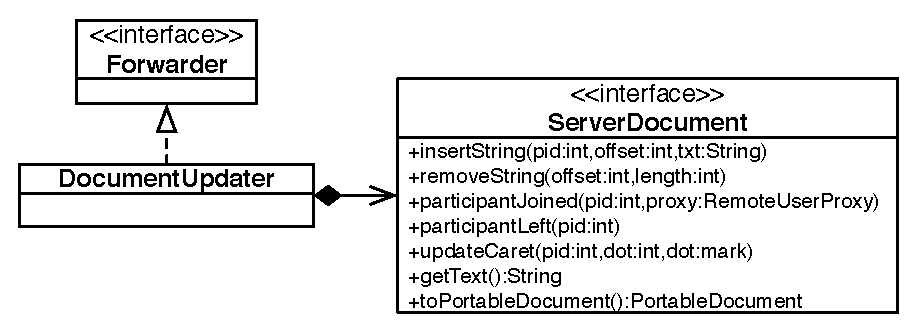
\includegraphics[width=15.00cm,height=5.08cm]{../images/finalreport/collaboration_documentupdater_uml.eps}
 \caption{DocumentUpdater and ServerDocument}
 \label{fig:collaboration.documentupdater}
\end{figure}

The \texttt{Document\-Updater} is set as the default forwarder for the
\texttt{Composite\-Forwarder\-Impl}. This has an important implication. If the
\texttt{Server\-Document} does not accept the operation (e.g. if the insertion
index is wrong), the \texttt{Failure\-Handler} is notified. The default
implementation of the \texttt{Failure\-Handler} (the class 
\texttt{Server\-Logic\-Impl}) removes the sender of the failing operation
from the session and notifies all the other participants that the participant
left (\texttt{send\-Participant\-Left}).


\subsection{Server Document}
\label{sect:archoverview.serverdocument}
The \texttt{Server\-Document} is used by the server to keep an up-to-date
copy of the document that can be sent to users that want to join the
session. The class diagram of the \texttt{Server\-Document} can be found
in the section about the \texttt{Document\-Updater} (see figure 
\ref{fig:collaboration.documentupdater}.

The \texttt{to\-Portable\-Document} method creates a snapshot of the document
that can be sent to the \texttt{send\-Document} method of the 
\texttt{Participant\-Connection}. The \texttt{get\-Text} method allows to
retrieve the plain text of the document. The other methods are used to update 
the document.

The default implementation extends the \texttt{Abstract\-Document} of Swing.
It uses the \texttt{Element} interface from Swing to model the fragments
of the document. Each continous block of text that belongs to the
same participant is an element. This element structure has to be kept
up-to-date if text is inserted and removed. The participant id of each
fragment is kept as an attribute in the \texttt{Element}'s 
\texttt{Attribute\-Set}.


\subsection{Participant Connections}
In figure \ref{fig:collaboration.serverflow} we have shown the basic flow
of messages in the session server from \texttt{Participant\-Port} to
\texttt{Composite\-Forwarder} to \texttt{Participant\-Forwarder} to
\texttt{Participant\-Connection}. However, that figure does not contain
all the details. The part with the \texttt{Participant\-Connection} is
a bit more complex as figure \ref{fig:collaboration.participantconnection}
shows:

\begin{figure}[H]
 \centering
 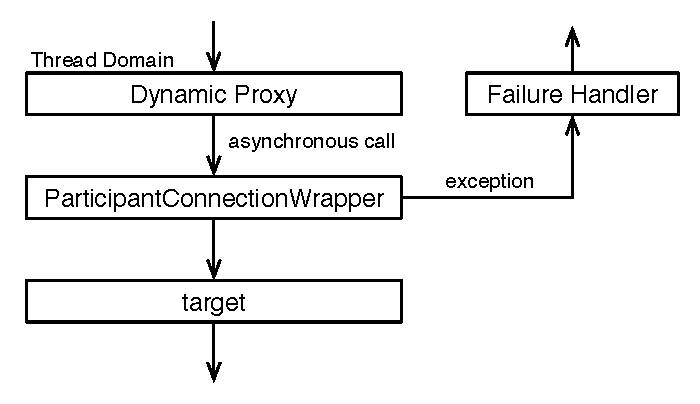
\includegraphics[width=11.29cm,height=6.28cm]{../images/finalreport/collaboration_participantconnectiondetails.eps}
 \caption{Detailed view of ParticipantConnection handling}
 \label{fig:collaboration.participantconnection}
\end{figure}

\texttt{Participant\-Connection}s passed to the collaboration layer
(either when joining or accepting an invitation) are wrapped with a
dedicated thread domain (see appendix \ref{chapter:threaddomain}). This
thread domain is called \emph{outgoing} thread domain.

As we have shown in the chapter about the algorithm (see chapter 
\ref{chapter:algorithm}), the processing of requests must be serialized
at the server. However, sending the transformed request back to the
other participants can happen concurrently. The session server can process
the next request. If we would not take care that the transformed requests
are sent concurrently, then a possibly slow network connection could slow
down the processing of requests at the server and thus the whole session.

In figure \ref{fig:collaboration.participantconnection} the first object
is the dynamic proxy created by the thread domain.
The invocation on the immediately following 
\texttt{Participant\-Connection\-Wrapper} is executed by the worker thread
of the thread domain. The wrapper passes the invocation to the target
connection. If the target connection throws an exception, it is caught
by the wrapper and an object implementing the \texttt{Failure\-Handler}
interface is invoked (see section \ref{sect:collaboration.failurehandling}).

Besides notifying the failure handler, the wrapper replaces the target
connection with a null object, an object implementing the
\texttt{Participant\-Connection} interface that simply ignores all the 
method invocations. This is done because it could be that in the
queue of the thread domain, there are still some method invocations for
that target connection. Instead of invoking methods on the target again
that result most likely in another exception, the target is replaced
and remaining invocations are simply discarded. We consider a
connection that has thrown an exception as dead, i.e. it can not be used
any longer.

There is also a \texttt{Publisher\-Connection\-Wrapper} that serves the
same purpose for \texttt{Publisher\-Connection}s as the
\texttt{Participant\-Connection\-Wrapper} does for 
\texttt{Participant\-Connection}s. For details about 
\texttt{Publisher\-Connection}s check the section 
\ref{sect:collaboration.publisherconnection}.


\subsubsection{Publisher Connection}
\label{sect:collaboration.publisherconnection}
\begin{figure}[H]
 \centering
 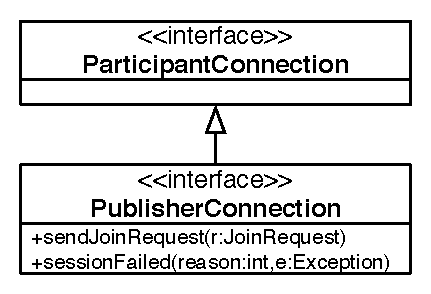
\includegraphics[width=6.74cm,height=4.41cm]{../images/finalreport/collaboration_publisherconnection_uml.eps}
 \caption{PublisherConnection Interface}
 \label{fig:collaboration.publisherconnection}
\end{figure}

The \texttt{Publisher\-Connection} extends the \texttt{Participant\-Connection}
interface with methods that are only available for a connection to the
publisher. The \texttt{session\-Failed} method is called when there is
a serious error in the session logic, which does not allow any recovery.
The session is then no longer usable and the document no longer published.

The \texttt{send\-Join\-Request} method sends a join request to the
publisher of the session.

The default implementation of the \texttt{Publisher\-Connection} interface
is the class \texttt{Published\-Session\-Impl}. 


\subsubsection{Failure Handling}
The \texttt{Participant\-Connection\-Wrapper} wraps a 
\texttt{Participant\-Connection}
and catches exceptions thrown by the target connection. If the target throws
an exception, the \texttt{Failure\-Handler} is called.

A failing \texttt{Participant\-Connection} expells the concerned participant
from the session.



\subsection{Usage of ThreadDomains}
\label{sect:collaboration.threaddomains}
The server logic uses \texttt{Thread\-Domain}s extensively. To learn about
\texttt{Thread\-Domain}s read the chapter \ref{chapter:threaddomains}.

\subsubsection{Incoming ThreadDomain}
As noted above, only one thread may access the server logic transformation
section at any time. Now, instead of using synchronized statements or
locks, we use thread domains to ensure that only one thread accesses the
server logic at any given moment. How can this be achieved? By wrapping
all incoming references with a \texttt{Single\-Thread\-Domain}. The possible
incoming references are:
\begin{itemize}
 \item all \texttt{Participant\-Port} instances
 \item \texttt{Server\-Logic}
 \item \texttt{Failure\-Handler}
 \item \texttt{Invitation\-Port}
\end{itemize}

This technique allows to solve two problems: first, the transformation must
be serialized and second, the caller does not have to wait for the
transformation to be completed.



\section{Miscellaneous}

\subsection{Acknowledge Strategies}
\label{sect:archoverview.acknowledgestrategies}
In the discussion of the algorithm 
(see section \ref{sect:algorithm.outgoingqueue}) we have noted that
in some situations the outgoing queues of the \emph{Jupiter} algorithm can 
grow indefinitely. To avoid this situation, a site that does not generate
requests on its own but receives requests from the other site should acknowledge
from time to time the messages processed from the other site in order to 
avoid that the queues grow too much. Acknowledge messages are rather simple.
They consist of the local site id as well as the local timestamp, which is
used by the other site to discard acknowledged messages from the outgoing
queue.

The collaboration layer uses objects implementing the 
\texttt{Acknowledge\-Strategy} interface to determine when to send 
acknowledge messages. This is a classical implementation of the
\emph{Strategy} pattern. The strategy itself does not know how exactly to 
send an acknowledge message. This is left to an object implementing the
\texttt{Acknowledge\-Action} interface, which has a single \texttt{execute}
method that is invoked by the strategy whenever it thinks it is
time to send an acknowledge message.

\begin{figure}[H]
 \centering
 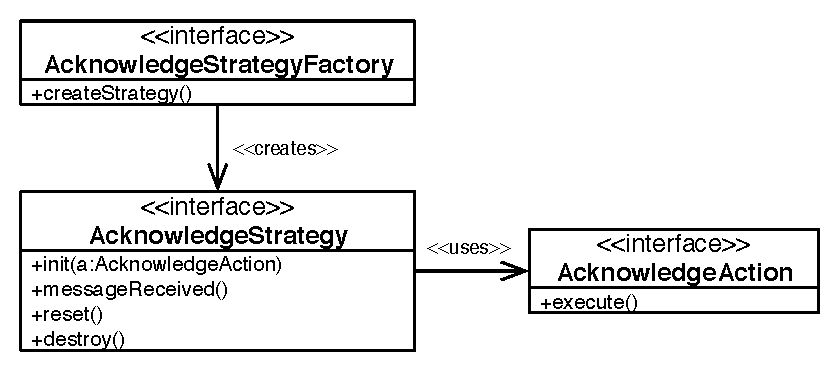
\includegraphics[width=13.65cm,height=5.72cm]{../images/finalreport/collaboration_acknowledge_uml.eps}
 \caption{AcknowledgeStrategy and related interfaces}
 \label{fig:collaboration.acknowledge}
\end{figure}

The strategies must be initialized with an action through the \texttt{init}
method. Code that uses an \texttt{Acknowledge\-Strategy} should call
\texttt{reset} whenever a message with a timestamp in it is sent to the
other site. Such a message makes sending acknowledge messages useless, as the
sent message already contains a timestamp. If a message is received from
the other site, the \texttt{message\-Received} method should be called.

Acknowledge strategies can decide when it is time to send an acknowledge
message. A possible strategy is to send an acknowledge message back to the other
site whenever a certain number of messages have been received (this is
the strategy used by the \texttt{Counting\-Acknowledge\-Strategy}). In that
case, the \texttt{reset} method resets the message counter to zero.

Another strategy could be based on a timer that fires after 60 seconds during
which no messages have been sent. The \texttt{reset} method in that
case would simple restart the timer.

The \texttt{Acknowledge\-Strategy\-Impl} combines both strategies described
above. The timer is just started when there has been a received message.

At the moment, ACE uses the simple message counting based implementation and not
the more complex and precise combined strategy. The timer based strategy
alone did not prove to be good enough, because potentially many messages
can be received in the timeout period.

\texttt{Acknowledge\-Strategy} objects are created by corresponding factories.
The interface implemented by this factories is named
\texttt{Acknowledge\-Strategy\-Factory}.


\subsection{Algorithm Wrapper}
The collaboration layer uses an extended \texttt{Algorithm} interface to support
handling of awareness information. This extended interface is called
\texttt{Algorithm\-Wrapper}.

\begin{figure}[H]
 \centering
 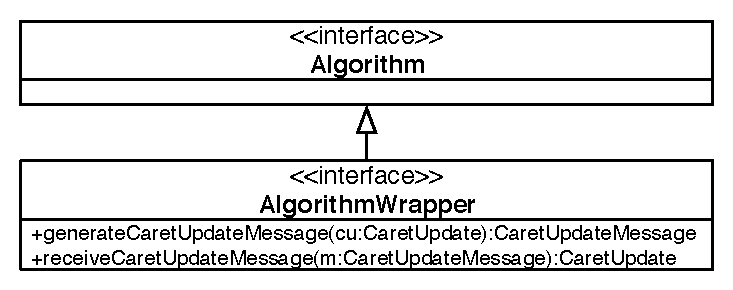
\includegraphics[width=11.85cm,height=4.34cm]{../images/finalreport/collaboration_algorithmwrapper_uml.eps}
 \caption{AlgorithmWrapper Interface}
\end{figure}

The two additional methods, \texttt{generate\-Caret\-Update\-Message} and \texttt{receive\-Caret\-Update\-Message}, are used to generate messages
to send updates of the local caret to the session and to receive such updates
from the session. The two additional objects used are \texttt{Caret\-Update}
and \texttt{Caret\-Update\-Message}. They correspond to the \texttt{Operation}
and to the \texttt{Request} interface.

\begin{figure}[H]
 \centering
 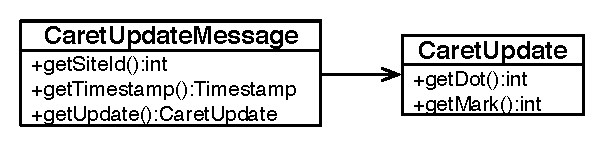
\includegraphics[width=8.89cm,height=4.73cm]{../images/finalreport/collaboration_caretupdate_uml.eps}
 \caption{CaretUpdate and CaretUpdateMessage}
\end{figure}

A \texttt{Caret\-Update\-Message} consists of the site id of the sender, the
timestamp at the sender's site, and a \texttt{Caret\-Update} object. The
\texttt{Caret\-Update} has a \texttt{dot} and a \texttt{mark} property. The
\texttt{dot} specifies the position of the insertion point, \texttt{mark} 
specifies the end of the selection. If both \texttt{dot} and \texttt{mark} are 
equal, nothing is selected. 


\subsection{Hosting ServerLogic}
Nothing in the design of the whole server logic prevents it to be used outside
of ACE. All incoming requests pass through a \texttt{Participant\-Port}, all
outgoing through a \texttt{Participant\-Connection}. So the server logic
is totally agnostic about the fact that the publisher is running inside
the same Java Virtual Machine. So, through the introduction of few additional
interfaces it would be possible to host the server logic on a different
computer. This is not supported at the moment by ACE but it would be
a minor feature to implement the server part.
